\documentclass[a4paper]{article}

%\usepackage[cm]{fullpage}
\usepackage[T1]{fontenc}
\usepackage[english]{babel}
\usepackage{textcomp}
\usepackage{multirow}
\usepackage{float}
\usepackage{fancyhdr}
\usepackage{pdfpages}

\usepackage{hyperref}
\hypersetup{
	pdfauthor = {Christian Wemstad},
	pdftitle = {eh2730: Procurement Project Plan},
	pdfsubject = {EH2730},
	pdfkeywords = {Procurement, elicitation, analyzation, verification and validation},
	pdfcreator = {LaTeX with hyperref package},
	pdfproducer = {latex}
}

\usepackage{graphicx}
\usepackage{amsmath}

\title{Assignment I: Procurement Project Plan for a WOMS-system}
\author{Henrik Sohlberg <\href{mailto:hsoh@kth.se}{hsoh@kth.se}> %
\and Christian Wemstad <\href{mailto:wemstad@kth.se}{wemstad@kth.se}> %
}

\fancyhf{}
\fancyhead[LE,RO]{\slshape \rightmark}
\fancyhead[LO,RE]{\slshape \leftmark}
\fancyfoot[C]{\thepage}

\begin{document}
\pagestyle{empty}
\maketitle

\newpage
\section*{Version table}
\label{sec:version_tabel}
\begin{table}[H]
	\centering
	\begin{tabular}{|l|l|l|}
		\hline
			\textit{Version} & \textit{Change log} & \textit{User}\\
		\hline
		     v. 1 & First version & Mr. Wemstad and Mr. Sohlberg \\
		\hline
	\end{tabular}
\end{table}
\newpage       
\tableofcontents
\newpage
\pagestyle{fancy}
\setcounter{page}{1}
\section{Background}
\label{sec:background}
This document is a project plan for the procurement project of ''The ACME WOMS project''. The ''The ACME WOMS project'' project will, if executed, implement a new digital system in the current ACME system collection. This system will be a Work Order Management System (WOMS) targeted to optimize proactive/reactive maintenance and the customer support process, in terms of costs and efficiency.

The background for this procurement project is that the company, ACME, has an outstanding economic issue, which has been a problem the company for a long time. The company has located a low profitability, which they think is an indicator that there may be sub-optimal solutions within the company. ACME has also analyzed the costs of the company and located that one of the biggest cost expenses are the customer support team. Furthermore, recently a new legislation was taken in action enacting a penalty fee for outages longer than 12, increasing the pressure to an already strained budget . The management department believes that cost reductions can be made in the maintenance and repair section if a better control system would be present. 

\subsection{Prior Work}
\label{sub:prior_work}
When the problems in the company was discussed some prior work was conducted to understand the magnitude of the situation. The first thing that has been executed is a survey regarding costs in different companies in this line of work. This survey indicated that ACME's costs were noticeably larger than their business rivals.

When the company realized that what they needed was WOMS, a brief investigation was made. This investigation resulted in the document, Appendix B, see section 1.2. The document explains what a WOMS system is and how it could benefit the company.

For current and upcoming systems, the organization has established a number of principles:
\begin{itemize}
\item Apply open standards when applicable
\item All data flows from ACME hosts to and from other networks (e.g. Internet) should pass through ACME's network boundary firewall proxy
\item For the ERP system, no modifications are allowed
\end{itemize}

These principles will be followed in this project. 
 
\subsection{Reference Documents} 
\label{sub:reference_documents}

This document is the result of the need for an integration plan for a WOMS system. This need is to be found in the Assignment I document. Information about the current ACME's company structure, IT-systems, business model and business system are collected from \textbf{Appendix A}\cite{A}. A brief introduction to how a WOMS system could be integrated into the current ACME system and what effect this might give is also stated in \textbf{Appendix A}\cite{A}. General information about what a WOMS system is are collected from \textbf{Appendix B}\cite{B}.

\subsection{Vision Statement}
\label{sub:vision_statement}
For ACME who deliver electrical power to factories and households, where the main costs are maintenance and customer support, the WOMS, a COTS software integrated with other systems in the organization, will enhance how proactive and reactive maintenance is functioning and how information can be provided to customers. 

Unlike existing work procedures that do not offer the ability to control neither how to dispatch work orders nor to follow up and reduce costs related to maintenance work, the WOMS product will fulfill not only how to control and optimize the maintenance function, but also enable ACME's customer support to provide better and more up-to-date information to customers. 

\subsection{Constraints}
\label{sub:constraints}

This project's focus lies on implementing a WOMS system into the existing IT-system that ACME has. Anything that is not directly related to this project or not specified in this document will NOT be included in this project.  I.e. during the prior-work of this procurement-project it has come to the company's attention that the support responsibility of the NIS and SCADA/DMS should be moved to the IS/IT department instead of the Operations department, this will NOT be included in this project. 

\subsection{Glossary}
\label{sub:glossary}

\begin{table}[H]
	\centering
	\begin{tabular}{|p{2cm}| p{3cm} |c| p{3cm} |}
	\hline
		\textit{Term} & \textit{Definition} & \textit{Aliases} & \textit{Example} \\
	\hline 
		
		WOMS	 & Work Order Management System & - & \\ \hline
		
		ACME	 & The company for which this procurement project is being executed& The Company & \\	\hline
		COTS	 & Commercial Of The Shelf & - & \\ \hline
		Project team & The core group of people responsible for this project & - & \\ \hline
		Junior Consultants & 2 members of the consultants agency responsible for this document, also members of the Project team & - & \\ \hline
		URD & User Requirements Document & - & \\ \hline
		NIS	& Network information system & - & \\	\hline	
		SCAD	A & Supervisory Control And Data Acquisition & - & \\  \hline
		DMS & Distribution Management System & - & \\ \hline
		CCB	& Change Control Board & - & \\ \hline
		CCPP	 & Change Control Policies and Procedures & - & \\ \hline
		COO	& Chief Operations Officer & - & \\ \hline
		PDA	& Personal Digital Assistant & - & \\ \hline
		SVN & Software Versioning And Revision Control System & Apache Subversion & \\ 
		URD & User requirements document & - &\\
		SRS & Software Requirements Specification & - & \\  

	\hline
	
	\end{tabular}
	\caption{A glossary of terms used in the document}
\end{table}

\section{Goals} 
\label{sec:goals}
The goal and purpose with procuring a WOMS is to have a system that can dispatch, prioritize and monitor work orders. It should also provide analysis functionality such as statistics on the  HAHAHAHAHAAHHAHA

The main costs of ACME's business are maintenance, repair and construction and the survey (section 1.1) indicates those costs to be beyond industry average. The major goal of this project is to resolve this issue, lower the costs to industry average, increasing the competitive value of the ACME company. Within the same scope, another goal is to tackle the "12 hour outage penalty" issue by cutting the costs for this post in half. 

Another major cost can be found in the customer care division. A WOMS can support this process, providing function and service to improvement and optimization. Therefore, two goals will be lowering: the number of incoming ''customer complaining cases'', and the average time for each case.
\subsection{Business Goals}
\begin{itemize}
\item Reduce the expenses for the maintenance/repair/construction post to $<100\%$ of industry average, till 1 May 2016
\item Lower the costs for "12 hour outage penalty" cases by 50\% till 1 May 2015
\item A 30\% decrease of costs for the customer care team division
\item Replace 20\% of the manual process with automated within the customer care team
\end{itemize}

\subsection{Project Goals}
\begin{itemize}
\item Procure and install a Work Order Management System
\end{itemize}

\section{Organization}
\label{sec:organization}

\subsection{Stakeholders}
\label{sub:stakeholders}
First we analyze and categorize the stakeholders using Gottesdiener method "Stakeholder categories". As described in the figure all the stakeholders will be divided into three different sub categories, customers, users and others. When this is done all of the sub categories are further divided into two new underlying categories. When this is done, all the stakeholders have been assigned a category type. 

\begin{figure}[H]
	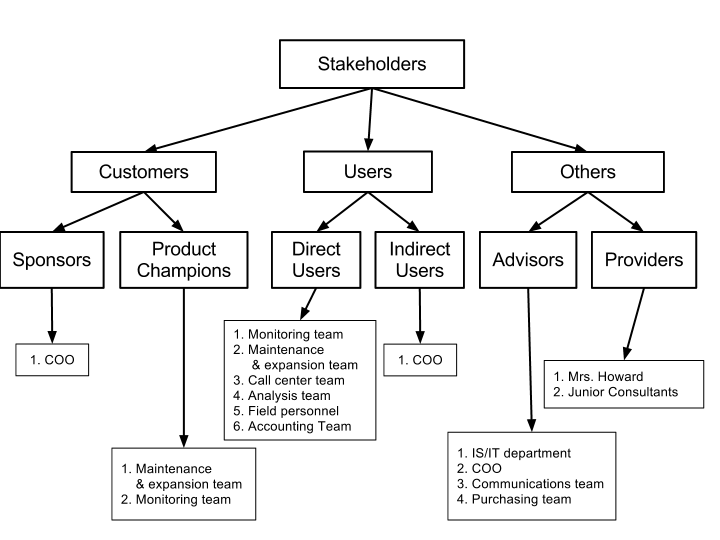
\includegraphics[width=1\textwidth]{images/stakeholder_categorization.png}
	\caption{Gottesdiener's model for categorizing stakeholders\cite{gott3}}
	\label{figure:stakeholder_categorization}                      	
\end{figure}

After all of the categorization of the stakeholders, a profilization of the stakeholder was conducted, see figure \ref{figure:stakeholder_profiles}. This was made to see what kind of involvement level, what interest, needs, concerns, constrains and success criteria each of the stakeholder categories have.

\begin{figure}[H]
	\includegraphics[width=1\textwidth]{images/stakeholder_profiles.png}
	\caption{Gottesdiener's model for profiling stakeholders \cite{gott3}}
	\label{figure:stakeholder_profiles}
\end{figure}

\subsection{Project Team}
\label{sub:project_team}
Finally a project team is created. This project team consists of the consultants from the consulting agency and 3 direct users. The direct users come from different parts of the company and will because of this have different input to the WOMS. From the stakeholder profilization table it stood clear that monitoring team, maintenance and expansion team, and call center team was the most involved in the changes the WOMS will make and were therefore specified as the most important stakeholder groups to have in the project team. Selected members to the project team are therefore:
\begin{itemize}
\item Mrs. Howard		- Consulting Agency
\item Mr Sohlberg	- Consulting Agency
\item Mr Wemstad	- Consulting Agency
\item Mrs Praxton		- Monitoring Team
\item Mr Flaxton		- Maintenance and Expansion Team
\item Mrs Braxton		- Call Center Team
\end{itemize}


We would have liked to have the field personnel in the project team as well but since this is a group of  external firms that support ACME with field personnel, this was not possible.

\subsection{Stakeholder Involvement}
\label{stakeholder_involvment}



\section{Project Model} 
\label{sec:project_model}
The purpose of this project is to find a WOMS system that will fulfill the goals specified in section 2. Since a WOMS system is a general specified system type that can be delivered from a multiple of different distributors the cheapest and simplest way to get one of these system is to buy a COTS system. One of the biggest challenges in selecting a COTS system is selecting a system that best fits the needs of the customer. To be able to do this type of selection we need to specify and analyze the requirements and needs the company have on this system. To successfully do this, this procurement project will embrace requirement engineering and the whole project have been divided into 4 phases, illustrated in figure \ref{figure:procure}. See section 5 for more information about the each phases in the model.
\begin{figure}[H]
	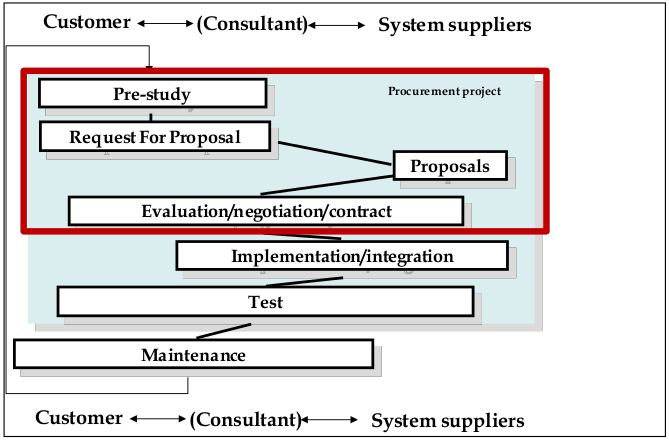
\includegraphics[width=1\textwidth]{images/procurement.png}
	\caption{Different phases in the procurement project, \cite{A}}
	\label{figure:procure}
\end{figure}
The table in section 4.1 describes each of the process in the procurement project model, figure \ref{figure:procure}. The \emph{Pre-Study} phase contain the five requirement engineering phases found in section 4.2. The estimated time for each process, phase, and activity is calculated according to the conditions: the time available is 1000 hour and the contract must be signed till 1 May 2013 \cite{I}. The time is determined by which stakeholders are involved in each activity, see section 3.2. Each activity is estimated with planning, execution, documentation, and re-iteration in mind.
\subsection{Table of Processes}
\begin{table}[!ht]
	\centering
	\begin{tabular}{|p{2cm}| p{3cm} |l| p{2cm} | p{1.1cm} | p{1.7cm}|}
	\hline
		\textit{Process} & \textit{Phases} & \textit{Time (h)} & \textit{Completion Date} \\
	\hline
		Pre-Study & Elicitation &  750 & 1 Mar\\
				  & Analysis & & \\
				  & Specification & & \\
				  & Validation & & \\
				  & Manage* & &\\ \hline
		Request For Proposal & - & 100 &10 Mar\\ \hline
		Proposals & - & 2&10 Apr\\ \hline
		Evaluation, &  &  140&1 May\\
		negotiation, & - & & \\
		contract & & & \\
	\hline
	\end{tabular}
\end{table}
* The \emph{Manage requirements} phase will continue after the pre-study is past \cite{gott7}.
\subsection{Table of Requirement Engineering Phases}
\begin{table}[H]
	\centering
	\begin{tabular}{|p{2cm}| p{4cm} |l | p{2cm}| p{1cm}|}
	\hline
		\textit{Phase} & \textit{Activities} &  \textit{Time} & \textit{Completion Date} & \textit{Time} \\
	\hline
		 		  & Facilitated workshop & 64& 24 Dec & \\ \cline{2-4}
		Elicitation & Exploratory prototype & 64&  1 Dec & \\ \cline{2-4}
				  & Interview & 4& 4 Dec &132\\ \cline{2-4} 
				  \hline
		Analysis & Process Map & 18& 6 Dec &\\ \cline{2-4}
				 & Context Diagram & 18& 10 Dec &\\ \cline{2-4}
				 & Business Policies & 18& 13 Dec &\\ \cline{2-4}
				 & Business Rules & 18& 16 Dec &\\ \cline{2-4}
				 & Use Cases & 30& 20 Dec &\\ \cline{2-4}
				 & Data Model & 12& 1 Jan &\\ \cline{2-4}
				 & One iteration  & 60& 20 Jan &\\ \cline{2-4}
				 & Prioritization & 24& 24 Jan & 198\\ \cline{2-4} 
				 \hline
		Specification & Create URD & 90& 2 Feb &\\ \cline{2-4}
				 & Create SRS & 90& 13 Feb &180\\ \cline{2-4}
				 \hline
		Validation & Peer Review& 18& 20 Feb Feb &\\ \cline{2-4}
				 & Iterate & 18& 1 Mar &36\\ \cline{2-4}
				 \hline
		Manage & Create CCCP\&CCB & 49& 1 March &\\ \cline{2-4}
				 & Manage changing requirements & 140& N/A &189\\ \cline{2-4} 
		\hline
	
	\end{tabular}
\end{table}

\section{Comments On The Project Model} 
\label{sec:comments_on_the_project_model}

\subsection{Pre-Study}
\label{sub:pre_study}
In the Pre-Study process there are five requirement engineering phase, described in 5.1.1-5.1.5. The input for this phase is prior work, see section 1.1. The output for this phase is a URD and a SRS.
\subsubsection{The Requirements Elicitation}
\label{subsub:the_requirements_elicitation}

The first step in the pre-study process is to elicitate all the requirements for the new WOMS software. This will be done through a series of different activities. The input to this phase will be the prior work, a vision statement and the stakeholder categorization as well as stakeholder profiles. The output will be a list of elicitated requirements. This phase is processed through the following activities which adapt to the model fig \ref{figure:elicitation}. 

\begin{figure}[H]
	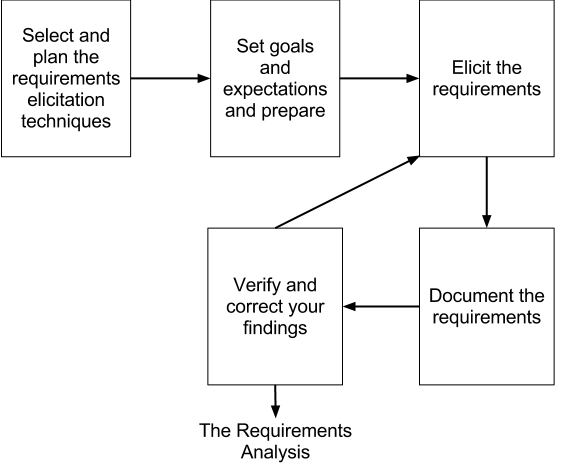
\includegraphics[width=1\textwidth]{images/elicitation_model.png}
	\caption{Gottesdiener's model for eliciting requirements\cite{gott3}}
	\label{figure:elicitation}
\end{figure}


A precondition for a successful requirements elicitation is to have planned for what techniques to be used (\textbf{Select and plan the requirements elicitation techniques}), and conduct preparations for each technique, specifying goals and expectations (\textbf{Set goals and expectations and prepare}). There are a number of different types of activities that can be used in the elicitation phase, \emph{Interviews, Facilitated Workshops, Exploratory Prototypes, Focus group, Observation, User Task Analysis, Existing Documentation Study} are the ones Gottesdiener describes in her book \cite{gott3}. Since our project is a COTS project, and the fact that we already have a clear specification about the functionality of the WOMS, the focus on the activities will be on figuring out the specific requirements for ACME and how the WOMS system should be used in their environment.

As for our first elicitation technique, we have chosen to use a \emph{facilitated workshop}. To decide who we shall invite to participate in this workshop we use the \emph{stakeholder categorization model}, specified in section 3. We have decided that the participants in this shall be 10 people, they will come from all of the different direct user groups, from the stakeholder categorization. In this workshop we will start by explaining what a WOMS is and the we let the participants try to define what they would like to see in such a product. The purpose of this activity is to gather information about what the direct users see as important in a WOMS system, we will also be able to get a brief understanding about how the users would like the system to look and interact with them.

The second technique to be used is exploratory prototype. We will design and build a prototype based on the outcome from the facilitated workshop. One of the purposes and the reason this technique is chosen is, as Gottesdiener proclaims \cite{gott3} - it is one of the best ways to validate requirements. This applies to figure 1 Verify and correct your findings. 

In addition to the two activities, we plan to interview the leftover stakeholders (the Communication Team and the IS/IT department) to get information of their needs. The output from the two earlier activities will act as a basis for interviews, as we believe it is likely that the, so far, elicited requirements will affect the technical specification - therefore the technical requirement (e.g. integration with other systems). This is the goal and the expectation for this method, to gain information like technical requirements and for example "... uncover conflicting software requirements." \cite{gott3}

\subsubsection{The Requirements Analysis}
\label{subsub:the_requirements_analysis}
The second process in the pre-study and planning stage is analysis of the requirements. The input is a list of elicited requirements, found in section \ref{subsub:the_requirements_elicitation}. The output will be a prioritized list of requirements and requirement models that will be used in later stages.

\begin{figure}[H]
	\centering
		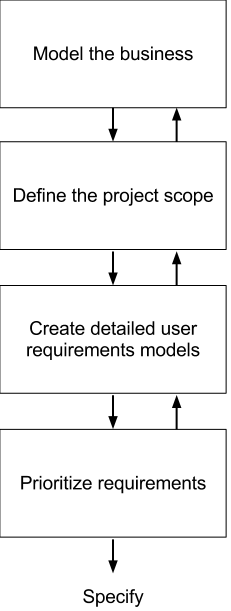
\includegraphics[width=0.3\textwidth]{images/analysis_model.png}
	\caption{Gottesdiener's model for analyzing elicited requirements\cite{gott4}}
	\label{figure:analysis}
\end{figure}

The analysis process can be divided into a 4-step model where the progress may move forward one step, as well as backward\cite{gott4}, visualized in figure \ref{figure:analysis}. The first step, \textbf{Model the business}, aims to map the functions and processes within the organization. This information will help in understanding how requirements will apply and affect the current business structure. The information will help uncovering new requirements and needs for changing processes, as well.
 
Next step, \textbf{Define the project scope}, is crucial. According to Singh \cite{projectsmart}, a unclear scope and poor planning is two common reasons to a project failing. Successfully defining the project scope will not only prevent the project and requirements to get out of hand, but it will also create better conditions to plan the project \cite{gott4}. 

With the business model and a definition of the project scope, the next step is to analyze the requirements in more detail. For this, Gottesdiener suggest to \textbf{Create detailed user requirements models}, multiple of them and iterate between them to reveal new facts and defects among the requirements.
        
When the models have been created, we will have bunch of user requirements. Next step in the Gottesdiener requirement analyze model is \textbf{Prioritize requirements}. This is necessary since there is a high probability that some requirements are unnecessary, interfering with each other, and are infeasible to include in the product\cite{Lec5}.  

Adapting this model, the activities in this process will be:
\begin{enumerate}
\item Process Map (\emph{Model the business}) 
\item Context Diagram (\emph{Define the project scope})
\item Business Policies (\emph{Define the project scope})
\item Business Rules (\emph{Create detailed user requirements models})
\item Use Cases (\emph{Create detailed user requirements models})
\item Data Model (\emph{Create detailed user requirements models})
\item Repeating 4-6 (\emph{Create detailed user requirements models} - iteration)
\item Prioritize using MoSCoW Scheme (\emph{Prioritize requirements)}
\end{enumerate}



A Process Map technique fulfill the purpose to model the business. The activity will yield manageable information over the business processes for the WOMS (based upon the elicitated requirements from section \ref{subsub:the_requirements_elicitation}). The output may also suggest improvements for other business processes \cite{gott4}, e.g. perhaps processes in the Call Center departement how they handle customers turn out to be improvable. Furthermore, Gottesdiener proclaims that one can use the output from a Process Map model as input to a Use Case and also to a Data Model activity\cite{gott4}.
      The Context Diagram (CD) together with the Business Policies (BP) activity are selected to define this project's scope. The BP activity is also motivated as ACME has stated and is following a number of policies/principles, see 1.2. In addition, output from the CD model can also be useful input to the Use Case activity and to the Data Model activity\cite{gott4} while the BP model support the Business Rules activity \cite{gott4}.
     The last three activities - Business Rules (BR), Use Cases (UC), and Data Model (DM) - are chosen because not only do they make use of output from earlier activities, they co-operate with each other, providing output as input, in a circular way. Activity relationships are illustrated in figure \ref{figure:business}
     
\begin{figure}[H]
	\centering
		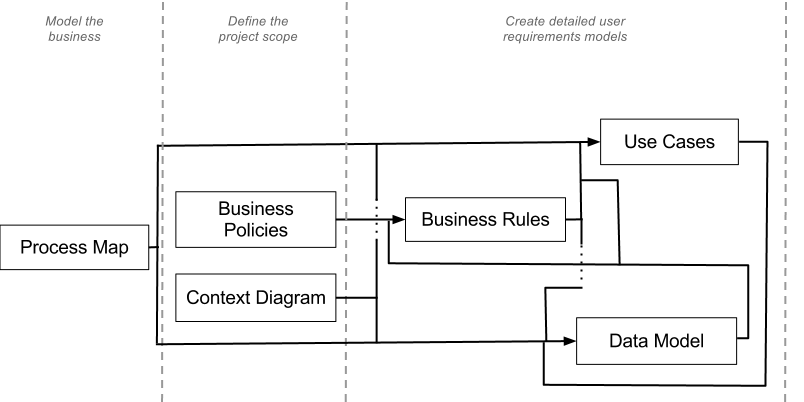
\includegraphics[width=1\textwidth]{images/model_the_business.png}
	\caption{Gottesdiener's model to model the business\cite{gott4}}
	\label{figure:business}
\end{figure}
     
We plan to perform two iteration in the Business Rules $\rightarrow$ Use Cases $\rightarrow$ Data Model activity sequence to make use of the property that they describe, in the big picture, the requirements for the same system. To iterate and updating respective models results in revealing new requirements, correcting and refining the "final" collection of requirements.

The last planned activity in this phase is Prioritization using the MoSCoW method. The motivation using this method: it is an uncomplicated, easy to use and far more useful than e.g. a traditional number system\cite{coleyconsulting}.

\subsubsection{The Requirements Specification}
\label{subsub:the_requirements_specification}

The third process is to specify all the requirements according to a uniform standard. The goal with this phase is to verify that the requirements that have been listed and analyzed are connected to the goals with the project and actually fulfill all of the specified goals\ref{sec:goals}. According to Gottesdiener\cite{gott5} this can be done by using a 4-steps model visualized in figure \ref{figure:specifications}. Gottesdiener specifies that the requirement. The input for this process will be the analyzed models from \ref{subsub:the_requirements_analysis} and the stakeholder profiles. The output will be a User Requirements Document (URD) and a Software Requirements Specification (SRS).

\begin{figure}[H]
	\centering
		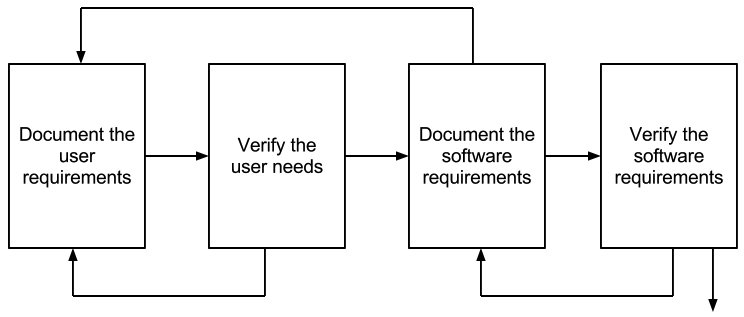
\includegraphics[width=1\textwidth]{images/specifications_model.png}
	\caption{Gottesdiener's model for specificaton of requirements\cite{gott5}}
	\label{figure:specifications}
\end{figure}

Gottesdiener's model starts with \textbf{Document the user requirements}, it aims to rewrite the requirements with the user as the audience and collect all the of these requirements in document. The second step in Gottesdiener's model is \textbf{Verify the user needs}; this part focuses on verifying that the requirements previously specified are complete and understandable from the different users point of view. Gottesdiener explains that specifying the user requirements in this way gives a more solid definition of the requirements, both in the the extra detail that this activity results in as well as the fact that this activity unifies all the requirements from the different stakeholder groups. \cite{gott5}. The final version of this document should give the user a good view of what they can expect of new system and how this new system will change the way they work\cite{gott5}. The step \textbf{Document the software requirements} aims on specifying the requirements from the software developers point of view. Furthermore will this document focus on functional requirements, quality attributes constraints and external interfaces to other systems\cite{gott5}. This document is also crucial for the requirements since it will work as a contract between the company and the external system suppliers delivering the WOMS \cite{gott5}. This document gives a much more in detail specification on what will be delivered than what would be possible with only a standard ("non requiremental") contract. 

When applying this model to this project we will assign the project team the responsibility to create the URD and the SRS. The project team will start creating this document by using the models created in section \ref{subsub:the_requirements_analysis}.  Given that the project team consists of 3 people from 3 different direct user categories, specified in the figure \ref{figure:stakeholder_categorization}, and the fact that the created models from section \ref{subsub:the_requirements_analysis} come from sound user requirements elicitations. This gives us confidence enough to not plan any extra meetings with the stakeholders in this activity and instead let the project team create this document on their own. This decision will result in time-savings without any major losses. When using Gottesdiener's model we will try to merge the first and the second step together, creating one unit that both document and verify the user requirements. The reason for doing this change is that we view this as such an iterative process, going back and forth between documenting and verifying, that they cannot be separated in an efficient manner.  

\subsubsection{The Requirements Validation}
\label{subsub:the_requirements_validation}
The fourth process the implementation can start is to validate that the specified requirements. In difference to the different validation steps in the other phases this phase focuses on how the requirements are specified. I.e "Did we get the requirements right?" rather than "Did we get the right requirement?". The purpose of spending time on this phase is therefore to validate that all the requirements are ambiguous and specified correctly. It is also important to find unnecessary, lacking or faulty requirements and to correct these\cite{gott6}. In is really important to understand that this phase should not be executed as a last step. It  should be an iterative process that progresses alongside with the other steps, constantly validating the current progress in the requirements engineering\cite{gott6}. Gottesdiener specifies the validation phase into 4-different steps, according to the figure \ref{figure:validation}\cite{gott6}. 


\begin{figure}[H]
	\centering
		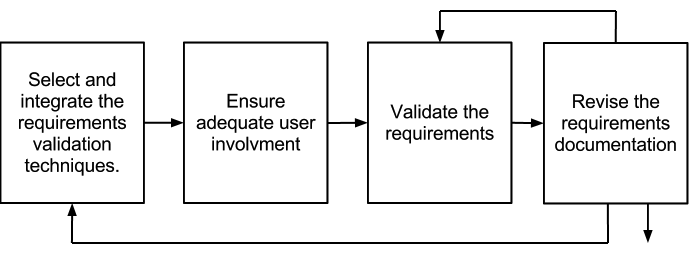
\includegraphics[width=1\textwidth]{images/validations_model.png}
	\caption{Gottesdiener's model for validation of requirements\cite{gott6}}
	\label{figure:validation}
\end{figure}


In the first step, \textbf{Select and integrate the requirements validation techniques}, the goal is to select the best techniques for the current stage in the requirements engineering process that most efficient validates the current progress. The second and third step, \textbf{Ensure adequate user involvement} and \textbf{Validate the requirements}, focuses on selecting the right stakeholders to be in the current validation method and executing the method. The last step in this model is \textbf{Revise the requirements documentation}. The focus here lies on using the result in from the validation to revise and update the documents, removing any found errors. The input to the validation phase, including the peer review, will be all of the current produced documents of the current produces documents. The output will be the same documents in a reviewed state\cite{gott6}.

The first method that will be used in this phase will be the Peer review method \cite{gott6}. The reason for selecting the Peer review method is because this method is specified to be used in the beginning of the requirements engineering process\cite{gott6}. The Peer review is executed using a small group (8-9 persons) of stakeholder. The stakeholders will be both from the users side of the system as well as from the system administrators. By having both these views in the validation of the new system we will be able to do what the users need and that it is possible to integrate the system in the current environment. The peer review meeting will be executed as a standard inspection peer review and will moderated by one person from the project team. After the peer review has been executed, the project team along with the moderator will revise the documents and update them when needed. The group will also specify what next validation activity will be.

\subsubsection{Manage The Requirements}
\label{subsub:manage_the_requirements}
The final process that needs to be completed before the request for proposal is the management of the requirements phase. Requirements engineering is an iterative process and the requirements for the system will constantly be affected by external factors, such as a new system environment or changing time or budget constraints. There is also a great risk for mistakes and other oversights throughout the whole requirement engineering phase. When the implementation project has started the concretization of the problem will result in finding these faults. Having a detailed described way of handling theses changes and faults are a crucial part of requirements engineering\cite{gott7}. Without it, there is a great risk of the project being delayed or even cancelled \cite{gott7}. By carrying out a good managements of the requirements these risks can be minimized and the survival of the project can be secured. 

This phase will be a constant work throughout the whole project and because of this there is no direct output that can be specified for this phase. The only actual output is new or changed requirements that more accurately describe the project and, of course, a successful project. The input to this phase will be any produced document about the project. Since the phase is about handling changes, anything can be relevant.

In this phase, there will be one main activity. This activity will be to investigate when changes that will affect the requirements happen and act accordingly. Before this activity can start there are some preconditions that have to be fulfilled\cite{gott7}. The first thing we need to do to fulfill these preconditions is to establish mechanisms for managing change requirements, this activity will result in a document called Change Control Policies and Procedures (CCPP). This document will, inter alia, specify how requirements changes will be recorded as well as how the software project aligns with the changing business needs. With this document the project will have a documented way on how to respond to changing requirements and ways to minimize the disruption to the project plan in whole when changes are needed. When specifying this document we will also create a Change Control Board (CCB). The CCB is a specialized group of stakeholders who are in charge when it comes to doing changes according to the CCPP. This group will consist of the members of the project team, \ref{sub:project_team}, and the COO. When the procurement project is finished and the implementation begins, the consultants in the project team will be replaced with members from the hired vendor. Since the CCB is responsible for the changes in requirements, it is in their interest to create time and budget for doing these changes.

The second precondition that needs to be fulfilled is understanding requirements lineage and relationships. To successfully do this we will construct a Requirements Trace Matrices (RTM). The RTM will specifies the correlation between software and implementation components, business goals and the requirements. With this type of document the CCB will have a greater control on what effects a change a requirement will have for both different software components and business goal. 

\subsection{Request For Proposal}
\label{sub:request_for_propsal}
When the phase of Pre-Study is finished, the next goal will be to create an Request for proposal (RFP). The purpose of the RFP is to, for the vendors, clearly specify what ACME wants from their new software, when they want in and how it should be delivered\cite{SPM34}. The RFP should be so clearly stated that this document is all the vendors need to make their proposal for the new system. 
When creating the RFP it is necessary to collect and summarize all the outputs from the Pre-Study and Planning phase, specifically the URD and the SRS document.The main output of this phase is a request for proposal document that in detail will explain all the needs and requirements for the software. To make a full and complete RFP it will also contain the vision statement, deliverables, a statement of approvals, type of contract, schedule and payment terms\cite{SPM3536}.

The stakeholders creating this document will be the junior consultants and Mrs. Howard. Validation and correction will be done by the COO of ACME in interaction with Mrs. Howard, since these are the 2 members of the project that are the most responsible.

\subsection{Proposal}
\label{sub:proposal}
When the RFP is clearly specified, it will be sent out to 
The goal of this phase is to retrieve different proposals so the one that best suits ACME's needs can be selected, by doing this we have a basis for ensuring that the best vendor can be selected. The input to this phase will be a request for proposal, delivered to the vendors. The output of this phase will be a group of different proposals delivered by the vendors. The junior consultants will be responsible for this phase, as well as contacting the vendors. No other stakeholders will be involved, since no decision making or discussion is needed in this phase.

\subsection{Evaluation, Negotiation and contract}
\label{sub:evaluation_negotiation_and_contract}
In this phase, the final phase of the procurement project, the goal of this phase is to find the best vendor and sign a contract with this vendor. The input to this phase will be the list of different proposals that are collected in the previous phase. The output will be a finalized contract, signed by both ACME and the selected vendor. 

This phase will use the whole project team when evaluating the different vendors and a light selection of which vendors to proceed with will be made. The resulting vendors will be presented to the COO and called to negotiations meetings. Further selection of vendors will be made and, if needed, extra negotiations meeting will be conducted. The negotiations meetings will be held by Mrs. Howard and the selections will be made by done by her and the COO. When the winning vendor has been elected, with a final contract specified by the negotiations, the contract will be signed by the vendor and the COO together with the Purchasing Team.

As specified in section \ref{subsub:manage_the_requirements}, the COO is a part of the CCB, he has therefore a very important role in the negotiation activity and in the creation of the contract. His role here is to ensure that the contract clearly specify how the management of the requirements will be handled after the contract is signed.
 
\section{Risk Analysis}
\label{sec:risk_analysis}
For probably every project, having a risk management strategy is of great importance because the occurrence of changes and unpredictable events lies in project management's nature \cite{k�lla?}. The primary focus of this project plan is on requirements. In this section, a risk analysis created according to Gottesdiener Requirement Risk Mitigation Strategy \cite{gott2}, is presented. 

\begin{table}[H]
	\centering
	\begin{tabular}{|p{2.5cm}| p{2.5cm} |p{2.5cm}| p{2.5cm} | p{2.5cm} |}
	\hline
		\textit{Risk Factor} & \textit{Probability of Risk} & \textit{Impact of Risk} & \textit{Risk Mitigation Strategy} & \textit{Team Member Responsible} \\
		
	\hline 
		Team Member Responsible & Low & Medium & - Revise activities involving a "difficult"-stakeholder, try find other suitable methods & Henrik Sohlberg \\ \hline 
		Developers adding unnecessary functionality & Mid & Low & - Put emphasis on creating a flawless URD and SRS combined with a clearly stated contract with vendor & Christian Wemstad \\ \hline 
		Requirements are constantly changing during the whole procurement project & Mid & Mid-High (the later the higher) & - Perform additional "define project scope"- methods
such as Event-Response table & Christian Wemstad \\ \hline 
		Unable to reach consensus between stakeholders during requirement prioritization phase & Low & Mid & - Make us of other  prioritization methods, e.g. "100\$ method", Requirements Prioritization based on Value, Cost, and Risk etc. & Henrik Sohlberg \\ \hline 
		Field personnel seriously lacks experience, e.g. handling a PDA, that a WOMS system requires & Low & High & 
- Educate and introduce them to the demanded technology, sufficiently, before they are involved in any requirement engineering processes & Henrik Sohlberg \\ \hline 



		
	\end{tabular}
\end{table}

\section{Document Rules} 
\label{sec:document_rules}

To easy understand what files are included in the project a unified way of writing, editing and handling documents, the following rule is stated. 

All the files shall have a version table in the beginning of the document and the current version of the file shall be specified in the end of the document name.

All files will be stored on ACME's own SVN server, using the standard backup system. Stakeholders outside the company will be given access to relevant parts of the SVN server.
 
\subsection{Document Standards}
\label{sub:document_standards}
The URD document will use the business standard PSS-05, specified by the European Space Agency\cite{PSS}. The SRS will be specified using IEEE STD 830-1998 \cite{IEEE}. Using these standard is for completeness and consistency reasons.The PSS-05 format will also add processes in how to write requirements and with this we can be certain that the requirements are specified correctly. Furthermore, using a well known standard will increase the readability for any reader already familiar with the bot the PSS-05 standard as well as IEEE STD 830-1998.

\addcontentsline{toc}{section}{References}
\begin{thebibliography}{99}     
	
\bibitem{gott2} \emph{Gottesdiener, Ellen. \textsl{"The Software Requirements Memmory Jogger" chapter 2}. GOAL/QPC, 2005}

\bibitem{gott3} \emph{Gottesdiener, Ellen. \textsl{"The Software Requirements Memmory Jogger" chapter 3}. GOAL/QPC, 2005}

\bibitem{gott4} \emph{Gottesdiener, Ellen. \textsl{"The Software Requirements Memmory Jogger" chapter 4}. GOAL/QPC, 2005}

\bibitem{gott5} \emph{Gottesdiener, Ellen. \textsl{"The Software Requirements Memmory Jogger" chapter 5}. GOAL/QPC, 2005}

\bibitem{gott6} \emph{Gottesdiener, Ellen. \textsl{"The Software Requirements Memmory Jogger" chapter 6}. GOAL/QPC, 2005}

\bibitem{gott7} \emph{Gottesdiener, Ellen. \textsl{"The Software Requirements Memmory Jogger" chapter 7}. GOAL/QPC, 2005}


\bibitem{SPM34} \emph{Gido, Jack. Clements, James P. \textsl{"Successful Project Management", edition 4, page. 34}. Cengage Learning, 2008}

\bibitem{SPM3536} \emph{Gido, Jack. Clements, James P. \textsl{"Successful Project Management", edition 4, page. 35-36}. Cengage Learning, 2008}    

\bibitem{A} \emph{The ACME Power Company: Appendix A}

\bibitem{B} \emph{Work Order Management Systems Basics: Appendix B}

\bibitem{I} \emph{Project plan for procurement project: Assignment I}

\bibitem{coleyconsulting} \emph{\textsl{"MoSCoW Prioritisation"} Gathered 2012-11-20} <\url{http://www.coleyconsulting.co.uk/moscow.htm}>

\bibitem{projectsmart} \emph{Singh, Manjeet. \textsl{"Rescuing Projects in Crisis: Project Turnaround Pointers"} Gathered 2012-11-20} <\url{http://www.projectsmart.co.uk/rescuing-projects-in-crisis.html}> 

\bibitem{IEEE} \emph{\textsl{"IEEE Recommended Practice for Software Requirements Specifications", IEEE Std 830-1998}  }

\bibitem{PSS} \emph{Mazza, Carlo. Fairclough, Jon. Melton, Bryan. de Pablo, Daniel. Scheffer, Adriaan. Stevens, Richard. \textsl{"Software Engineering Standards"}. Prentice-Hall International, 1994 } 

\end{thebibliography}
\clearpage
\appendix
\section{Stakeholder Elicitation Plan}
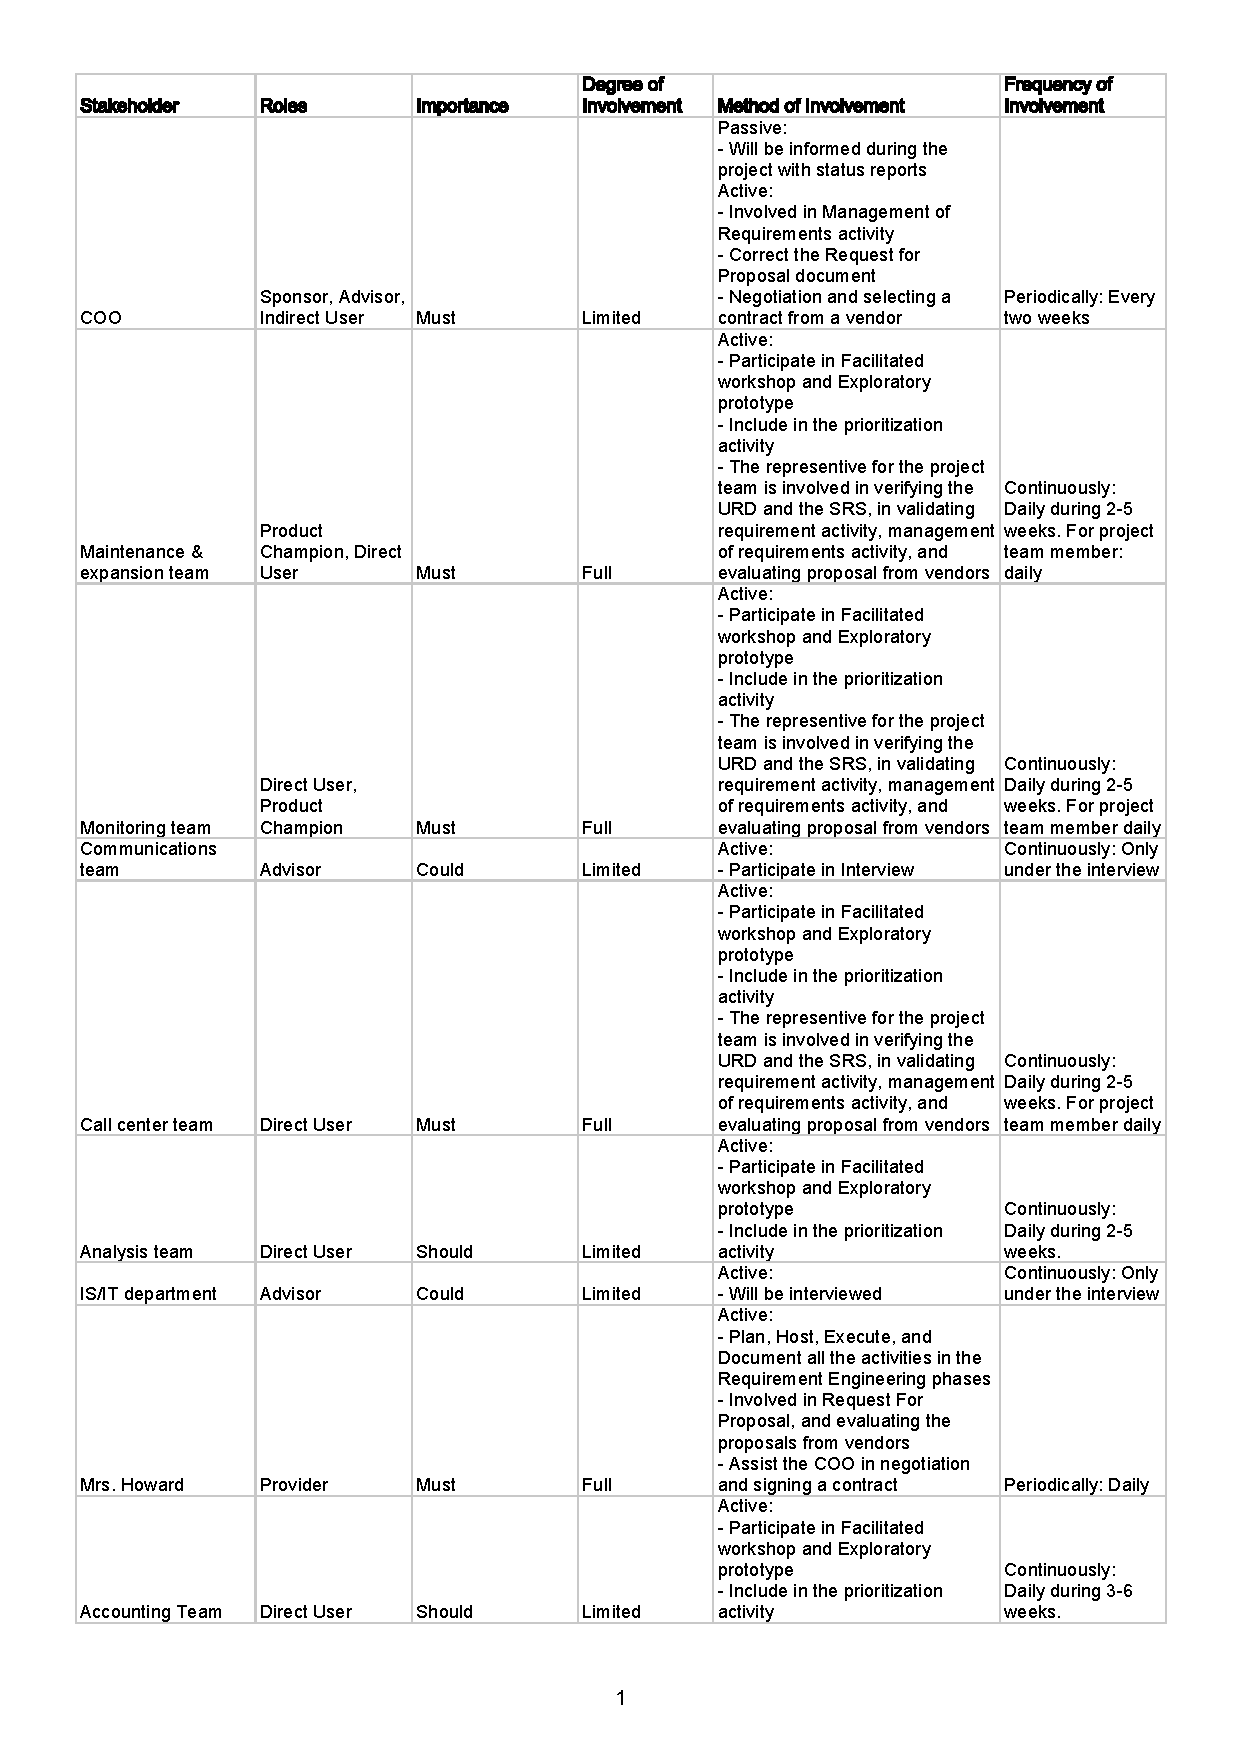
\includepdf[pages={-}]{appendix/stake_eli_plan.pdf}

\end{document}